%==============================================================================
%== template for LATEX poster =================================================
%==============================================================================
%
%--A0 beamer slide-------------------------------------------------------------
\documentclass[final]{beamer}
\usepackage[orientation=portrait,size=a0,
            scale=1.25         % font scale factor
           ]{beamerposter}

\geometry{
  hmargin=2.5cm, % little modification of margins
}

%
\usepackage[utf8]{inputenc}
% diminuir o tamanho da legenda das imagens
\usepackage[font=small,labelfont=bf]{caption}

% pacotes para fluxograma
\usepackage{tikz}
\usetikzlibrary{shapes,arrows}

\renewcommand{\figurename}{Figura}

\linespread{1.15}
%
%==The poster style============================================================
\usetheme{sharelatex}

%==Title, date and authors of the poster=======================================
\title
[24$^{o}$ Simpósio Internacional de Iniciação Científica da USP] % Conference
{ % Poster title
The Fate of Man-made Radionuclides in a Semi-Enclosed Basin
}

\author{ Silva, Danilo A.\inst{1} $\&$ Dottori, Marcelo\inst{2}
}
\institute[Instituto Oceanográfico - Universidade de São Paulo]
{
Instituto Oceanográfico da Universidade de São Paulo (IOUSP)\\ [0.2ex]
\inst{1} danilo2.silva@usp.br; \inst{2} mdottori@usp.br
}
\date{\today}



\begin{document}

\begin{frame}
%==============================================================================
\begin{multicols}{2}
%==============================================================================
%==The poster content==========================================================
%==============================================================================

\section{Introduction}

In a global scale, water reservoirs are used to dump material from power plants and
industries, where the biggest impact occur in areas with low circulation and water
exchange with open ocean. In the context of nuclear power plants, 96$\%$ are installed
closest to water bodies, using this waters in the cooling system. In Brazil, there is
two nuclear power plants in operation, located in the Almirante Alvaro Alberto 
Central Nuclear (AAACN), that captures and discharge water in the Ilha Grande Bay
(Figure~\ref{fig:areaestudo}), region with great touristic and social ambiental importance.

Understand the circulation patterns in this region is important to avaliate how the nuclear
material will disperse supporting the stakeholders, in the case of a nuclear leakage, such
as occurred in Fukushima, in 2011.

This study aims to investigate how wind and tide force the dispersion of these radioactive material in the
estuary system and where they will affect with greater impact.

\vspace{.1in}
\begin{figure}
\centering
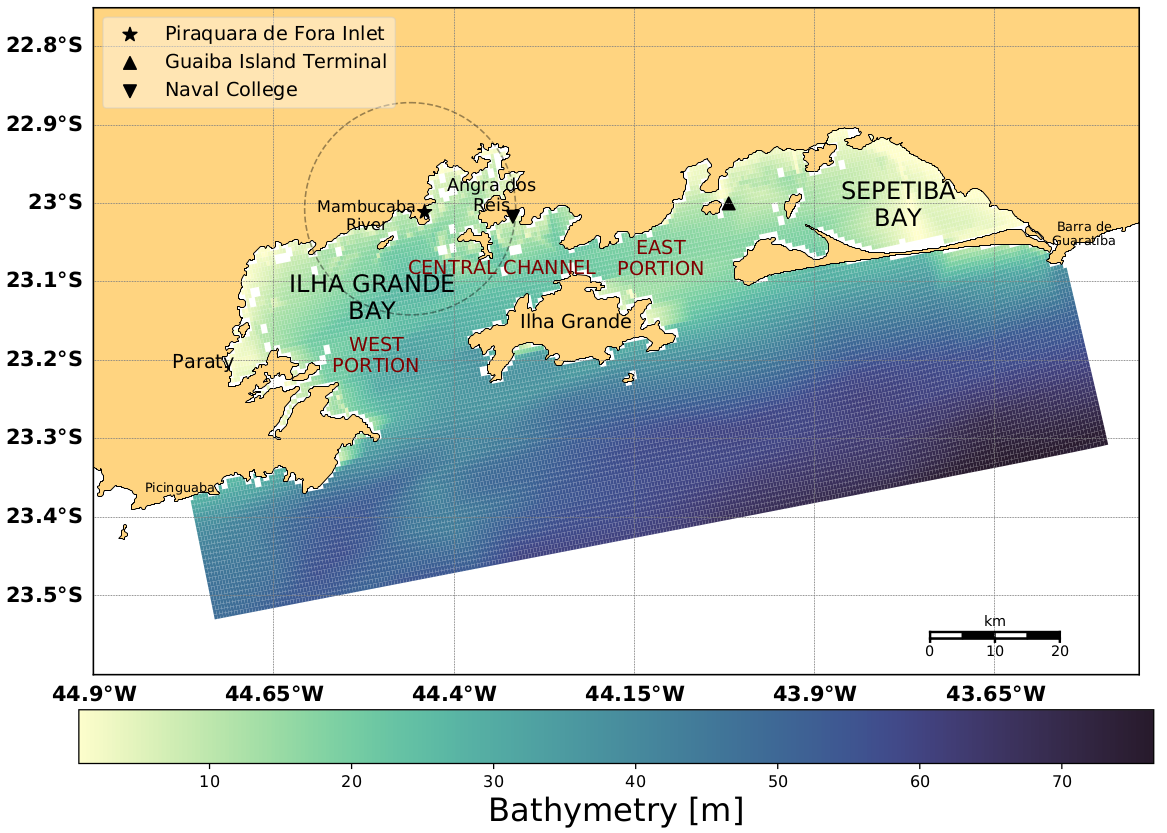
\includegraphics[width=0.8\columnwidth]{/home/tparente/danilo/mestrado/github/congressos/iwmo2018/figs/fig1.png}
\vspace{.1in}
\caption{The Ilha Grande and Sepetiba Bay domain used for ECOM model runs, showing bathymetry in meters. Several sites that are discussed in the paper are shown.}
\label{fig:areaestudo}
\end{figure}
% \vskip1ex
\vspace{-.5in}
% ===================================================================================================================
\section{Methods}

% Para determinar como o vento e a maré,
% principais forçantes, atuam na região, utilizou-
% se o \textit{Stevens Estuarine and Coastal
% Ocean Model}, ou sECOM.
% O modelo possui diversos módulos,
% onde ó módulo hidrodinâmico foi o utilizado
% para modelar a influência de cada variável
% na circulação da região.

\vskip1ex
\begin{figure}
\centering
\includegraphics[width=0.69\columnwidth]{/home/tparente/danilo/mestrado/github/congressos/iwmo2018/figs/diagramaTGFINAL1.png}
\vspace{.2in}
\caption{Scheme of the method applied in this work, where the read boxes represent input data, black boxes the modules from
ECOM and the blue boxes represent the experiments performed in this work.}
\label{fig:metodologia}
\end{figure}
\vskip1ex

\vspace{-.7in}
% ===================================================================================================================

\section{Results and Discussions}

\subsection{Wind v. Tide: Surface Circulation}

Was observed an intense eastward current in central channel in the Experiment I, reaching velocities closest
to 0.25 $m.s^{-1}$, while in the Experiment II such current reach a maximum of 0.23 $m.s^{-1}$, with a 
westward direction. The difference between those two experiments, considering the same wind's intensity,
may be cause by the open area available for southwesterly wind.
Finally, in the Experimet III, only with tides from TPXO 7.2, present the highest velocities,
concentrated in the eastern region of modelled domain, with maximum of 0.6 $m.s^{-1}$ during flood spring tide.

%\begin{itemize}
%	\item Direção da pluma é controlada pela direção do vento
%	\item Scenario I: intense eastward current in central channel, reaching velocities of 0.25 m/s
%	\item Scenario II: such current observed reach a maximum of 0.23 m/s, with a westward direction.
%	\item Scenario III: we observe the highest intensities in the domain, concentrated in the eastern region,
%	reaching 0.6 m/s in flood spring tide.
%	\item Mini Conclusion: western region dominated by wind-driven circulation and eastern region dominated by tidal-driven circulation.
%\end{itemize}

The results show that

%Talk about scenarios 5 and 6 (tides with typical winds in each experiment), highlightning regions more intense,
%direction of surface circulation.

%Quote Signori,1980a and 1980b, about intensity and direction of the surface currents registered in his work.

%Nota-se que os ventos de SW (Figura~\ref{fig:cenariosCirc}.b) apresenta correntes
%médias mais intensas quando comparadas ao cenário com ventos de NE
%(Figura~\ref{fig:cenariosCirc}.a), onde a geometria da área estudada
%favorece ventos de SW com uma maior superfície de contato. Este resultado é
%também obtido por [1], onde o transporte gerado por ventos do
%quadrante Sul foram maiores que o transporte por ventos do quadrante Norte.
%Entretando, ao observamos o cenário somente com maré (Figura~\ref{fig:cenariosCirc}.c),
%nota-se que esta forçante gera correntes 2 vezes mais intensas a leste do domínio.

% \vskip.5ex
\begin{figure}
\centering
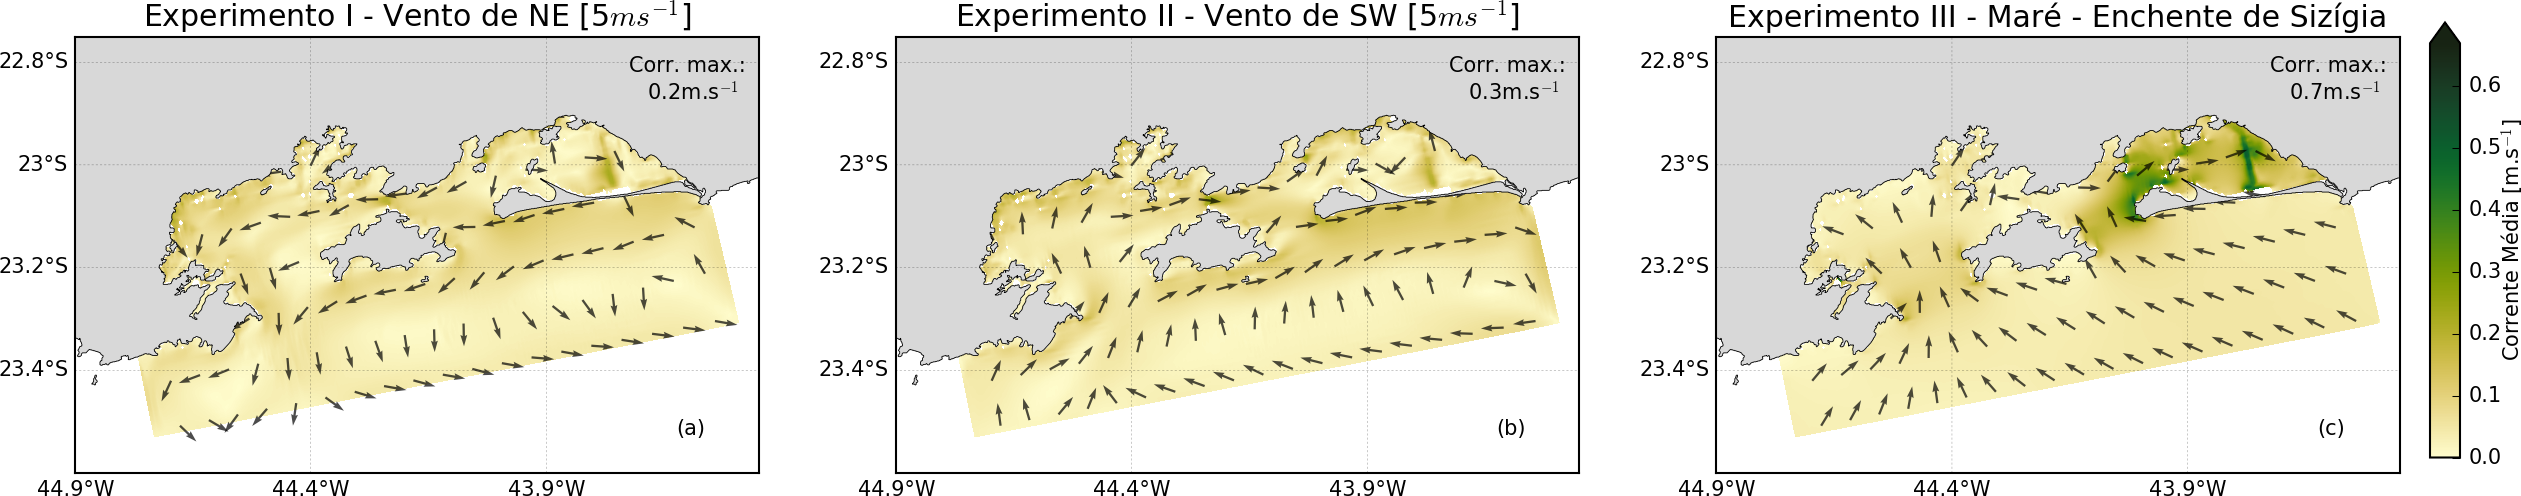
\includegraphics[width=1.\columnwidth]{/home/tparente/danilo/mestrado/github/congressos/iwmo2018/figs/figura1.png}
\caption{Corrente média nos cenários 1,2 e 3. Os painéis (a) e (b) representam o último instante modelado e (c), o instante da segunda
maré enchente de sizígia do período modelado.}
\label{fig:cenariosCirc}
\end{figure}

\vspace{-1ex}

Falar sobre como a direção da corrente é comandada pela direção do vento, apesar das variações de maré cheia e vazante,
logo a evolução da pluma de material nuclear será comandada pelo vento, enquanto que a dispersão comandada pela corrente
de maré.

%Comparando os experimentos 5 e 6, notamos que a maior diferença está na direção
%preferencial de evolução da pluma, que é comandada pela direção dos ventos em cada
%experimento. Entretanto, no experimento 5, os ventos de SW transportam o material
%radioativo para leste do domínio, atingindo regiões com correntes mais intensas devido à
%influência da maré e, desta forma, diluindo de maneira mais eficaz os radionuclídeos, em
%comparação ao experimento 6 que, para o mesmo instante de tempo, possui uma maior
% concentração do material na região oeste do domínio (Figura~\ref{fig:cenariosDispersao}).

\vskip1ex
\begin{figure}
\centering
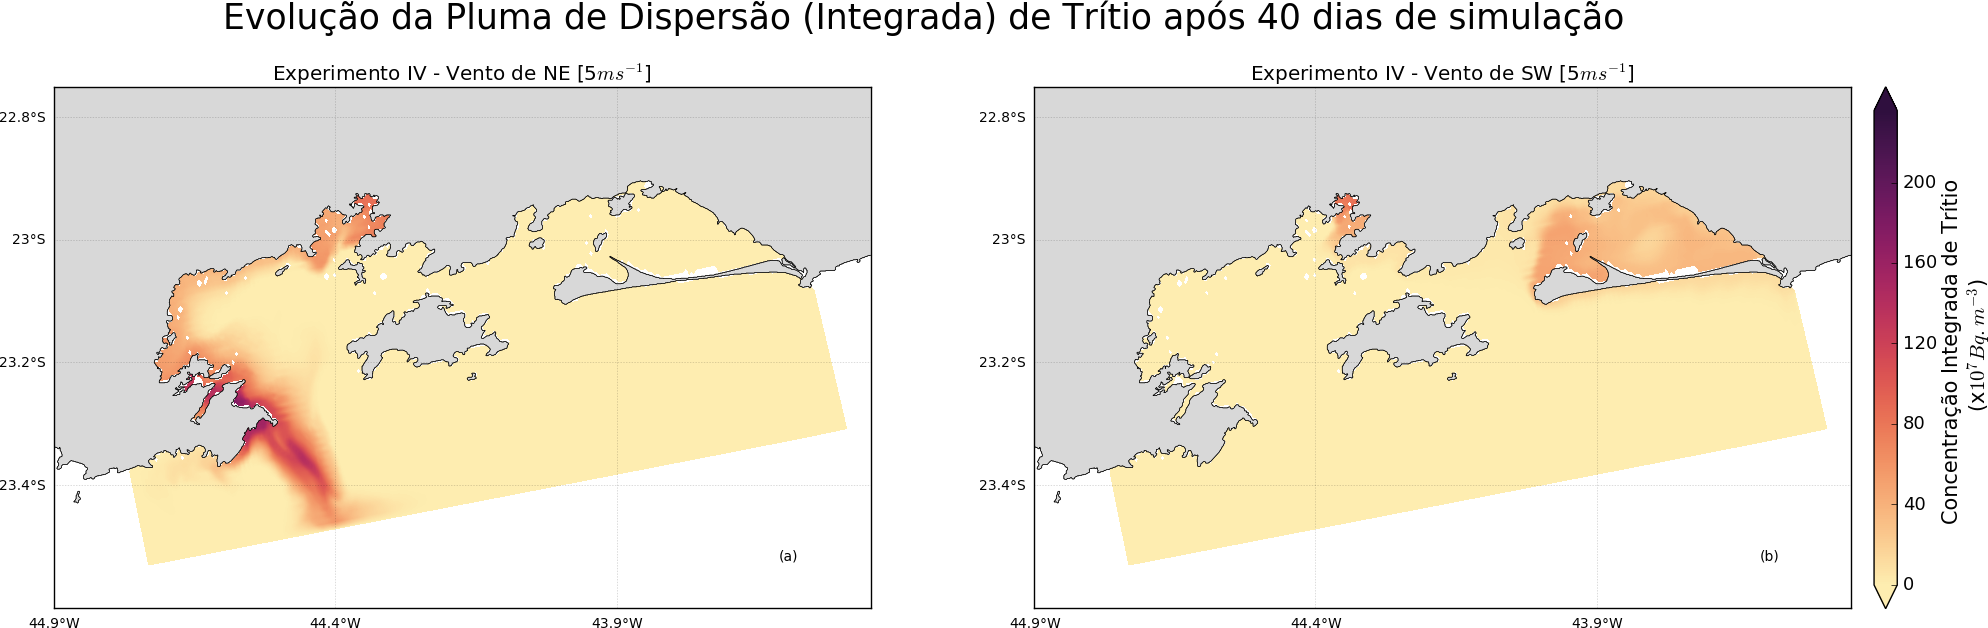
\includegraphics[width=0.99\columnwidth]{/home/tparente/danilo/mestrado/github/congressos/iwmo2018/figs/figura2_integrada.png}
\caption{Comparação entre os cenários 5 e 6, respectivamente, no instante correspondente a 40 dias de simulação, sendo
a concentração total na coluna.}
\label{fig:cenariosDispersao}
\end{figure}

\vspace{-1ex}

\subsection{Dispersion in a Scenario Under Nearest to Real Conditions}


%Quanto ao cenário 7 (Figura~\ref{fig:evolucaopluma}), observou-se que a evolução da pluma ocorre,
%preferencialmente, para leste do domínio, conforme no cenário 5, onde parte dela
%permanece por mais de 30 dias na Baía da Ribeira e outra parte é transportadapara regiões de
%correntes mais intensas, sendo rapidamente diluídas. Baseando-se nos cenários 5,6 e 7,
%estima-se que levaria mais de 60 dias para que grande parte do material fosse diluído na
%região, o que poderia acarretar em sérios problemas para a biota local, onde o material nuclear
%seria bio incorporado nos organismos e no sedimento, passando a fazer parte da cadeia alimentar.

%O tempo de permanência é melhor apresentado através da . Notamos
%que, de aproximadamente 150 horas a 500 horas, há uma grande concentração de material nuclear
%na Baía da Ribeira, região de descarte da Central Nuclear. A pluma alcança a região de
%Angra dos Reis a partir das 150 horas simuladas, permanecendo nessa região com uma
%concentração aproximadamente constante até o final da simulação.

\vskip-.4ex
\begin{figure}
\centering
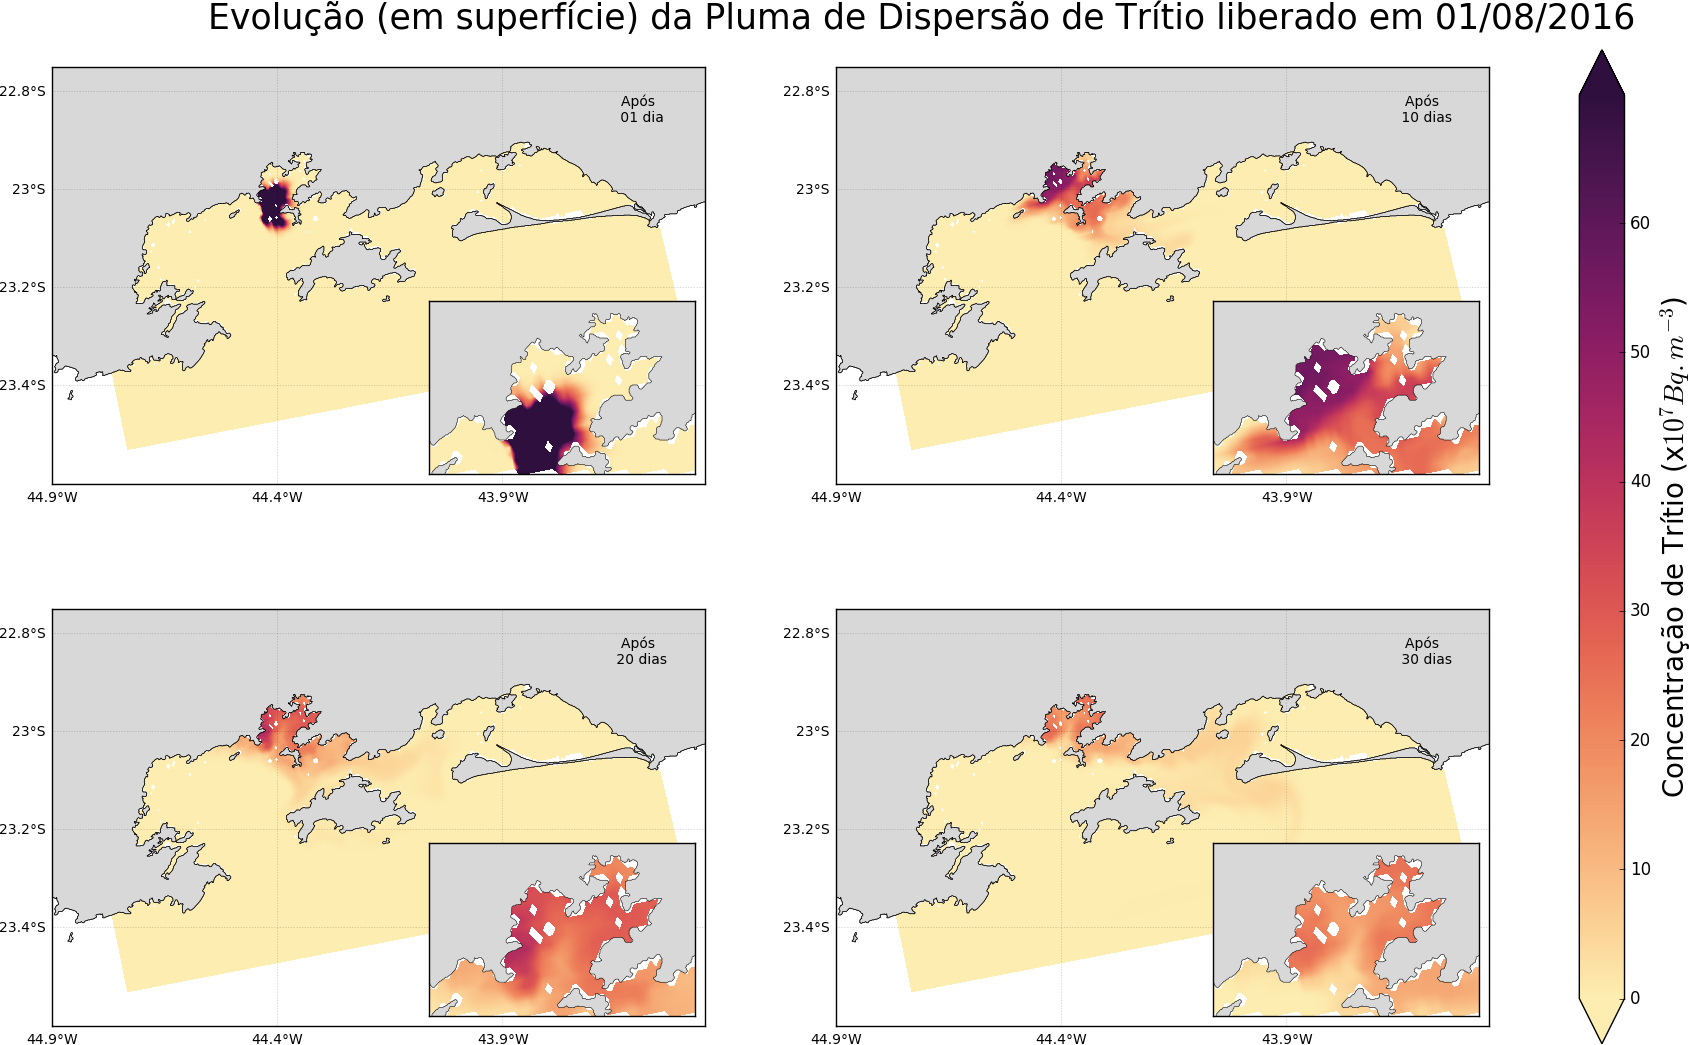
\includegraphics[width=0.9\columnwidth]{/home/tparente/danilo/mestrado/github/congressos/iwmo2018/figs/figura3_superficie.png}
\caption{Dispersão da pluma de material radioativo no cenário 6, os painéis representam, na ordem, os instantes de
6 horas, 10 dias, 20 e 30 dias após o vazamento.}
\label{fig:evolucaopluma}
\end{figure}
% \vskip2ex

Quote Rubens work, about concentration of radionuclides in surface sediment in Angra dos Reis.

% ===================================================================================================================
\vspace{-.5in}
\section{Conclusions}

Conclui-se que, em caso de vazamento nuclear na CNAAA, a presença do material
radioativo nas águas da região de estudo seria de, no mínimo, 60 dias, até uma redução a
níveis de concentração inferiores ao previsto na resolução no283 do CONAMA.
Além disso, as regiões de maior impacto seriam: Baía da Ribeira, ponto de descarte da
água e, dependendo do regime de ventos no instante do vazamento, a pluma poderá
alcançar regiões a oeste, como Paraty e Mambucaba, ou a leste, como Angra dos Reis,
Baía de Sepetiba e Marambaia.
Destaca-se que a pluma será melhor diluída ao atingir regiões a leste do
domínio estudado, onde a maré gera correntes mais intensas.

\end{multicols}

%==============================================================================
\end{frame}
\end{document}
